\chapter{Introducción}

Esta investigación tiene como objetivo transformar las instrucciones de algoritmos de grafos en una representación visual e interactiva a través de un videojuego. Esta representación se destina a estudiantes de informática, con lo que se puede evaluar si el uso de herramientas interactivas con feedback visual mejora tanto el aprendizaje como la motivación.

El trabajo implica presentar a estudiantes de ciencias de la computación (CS) un videojuego que exhiba grafos. En este juego, el usuario debe ejecutar las instrucciones de los algoritmos con la asistencia de elementos interactivos de caracter visual y auditivo.

El objetivo de esta investigación de tesis es identificar posibles diferencias en los niveles de motivación y comprensión de los algoritmos entre los estudiantes. Esto se medirá mediante una prueba que evaluará su conocimiento de los algoritmos de grafos.

El público objetivo son estudiantes de primer año de ciencias de la computación, aunque también es aplicable a estudiantes de ingeniería con conocimientos de programación. El requisito principal es que no hayan estudiado grafos previamente.

\section{Motivación}

La adopción de tecnologías digitales ha agilizado el acceso al conocimiento, permitiendo que estudiantes previamente excluidos ahora puedan acceder a la educación. Sin embargo, la educación en línea presenta desafíos propios \cite{UN2023ImpactDigitalTechnologies}. En este contexto, es crucial buscar metodologías que aceleren el aprendizaje con tecnologías adaptables, escalables y eficientes.

Se postula popularmente que la capacidad de atención de forma prolongada ha disminuido en las nuevas generaciones. Hay estudios que contradicen estas afirmaciones \cite{The_Role_of_Attention_Learning_Digital_Age}, indicando que las habilidades cognitivas de los estudiantes han cambiado, pero no necesariamente empeorado. Existen términos como ``doomsters'' y ``boosters'' \cite{Selwyn2014LookingF}, para descibrir la polarización entre estas miradas con respecto a la tecnología.

Existe consenso en que la tecnología y su portabilidad han incrementado notablemente la exposición de los estudiantes a distracciones \cite{Zimmerman2011HandbookOS, Wang2022ComprehensivelySummarizeDistractions}. El término "multitasking" se refiere al intento de llevar a cabo múltiples tareas simultáneamente. Aunque las personas tienden a creer que son capaces de realizar varias actividades de manera concurrente, diversos estudios han demostrado que esta práctica conlleva una disminución en la productividad y en el proceso de aprendizaje \cite{Domoff2019AddictivePU}. Con la generalización de los smartphones y la adopción de clases en línea, se ha observado un aumento significativo en la tendencia al multitasking durante las clases \cite{Wang2022ComprehensivelySummarizeDistractions}.

Una forma de distracción reconocida en la literatura es la interferencia motivacional, propuesta y explicada por Fries y Dietz \cite{Fries2007LearningMotivationalInterference}. Esta teoría postula que la motivación por los contenidos disminuye ante la presencia de estímulos más atractivos para la atención, tales como los smartphones. En este contexto, donde los estudiantes enfrentan la tentación de distraerse, resulta fundamental explorar estrategias destinadas a mantener su motivación y enfoque durante las clases.

Los videjuegos educativos destacan porque tienen potencial como una herramienta complementaria para la enseñanza, evaluación y entretemiento para los estudiantes. Entre sus beneficios se destaca la motivación. En \cite{Bisson1996FunInLEarningPedagogicalRole} se indica que para disfrutar una actividad, primero se debe permitir a la mente de un individuo percibir tal actividad como motivante. 

Yu et al. llevan a cabo una revisión sistemática de la literatura acerca de los efectos de los videojuegos educativos en el aprendizaje de los estudiantes y su motivación \cite{Yu2020TheEffectsOfEducationGames}. En relación con este último aspecto, el estudio señala que la incorporación de videojuegos educativos como recurso complementario impacta positivamente en la motivación y, además, mejora los logros académicos. Sin embargo, también destaca la existencia de investigaciones que contradicen esta afirmación, subrayando así la necesidad de llevar a cabo más estudios en esta área.

En el estudio mencionado, se asevera que el diseño del videojuego tiene una gran incidencia en el resultado final. Estos concluyen que las mecánicas, elementos visuales y narrativos tienen un efecto significativo, sugiriendo que los juegos educativos deberían implementar varios elementos de gamificación, como rankings, sistemas de recompensa, entre otros aspectos \cite{Yu2020TheEffectsOfEducationGames}.

Yu et al. \cite{Yu2020TheEffectsOfEducationGames} además mencionan una ventaja asociada a los videojuegos educativos, y es que pueden proveer servicios educacionales de alta calidad, flexible, portable y de bajo costo, incrementando las interacciones entre materiales de aprendizaje, estudiantes y profesores. Considerando lo anterior, se presenta una oportunidad para crear un videojuego educativo que enseñe algoritmos relacionados a grafos y analizar la percepción de sus usuarios.

En más del 50\% de los estudios citados anteriormente, se señala la falta de certeza con respecto a la percepción de los usuarios al jugar videojuegos educativos, concluyendo que se requiere profundizar la investigación. Por lo tanto, resulta pertinente emplear una prueba estandarizada que permita evaluar diversos diseños de videojuegos, abarcando distintas poblaciones objetivo, y cuyos resultados sean medidos conforme a un estándar uniforme. Con este propósito, se utilizó un formulario basado en el modelo MEEGA+ \cite{meegaplus} para evaluar la motivación de los estudiantes, y una prueba de conocimientos para medir su aprendizaje.


\section{Objetivo General}

El objetivo principal de este trabajo es medir el aprendizaje y la motivación de los estudiantes de computación al utilizar un videojuego educativo para instruir en algoritmos vinculados a grafo.

\section{Objetivos Específicos}

\begin{itemize}

\item Concebir una aplicación interactiva que visualice grafos y permita seguir los pasos relacionados con algoritmos que operan en dichos grafos. Esta aplicación debe tener elementos característicos de los videojuegos educativos.

\item Idear, desarrollar e implementar mecánicas de juego y una arquitectura de programación transferibles a otros videojuegos que instruyan en materias relacionadas con la programación.

\item Llevar a cabo una evaluación estandarizada para medir la percepción de los estudiantes respecto al videojuego creado.

\end{itemize}


\section{Marco teórico}

\subsection{Metodología de validación de videojuegos educativos}

Petri y Gresse von Wangenheim, en su trabajo \cite{HowGamesComputingEducationEvaluated}, llevaron a cabo una revisión de la literatura antes de desarrollar el modelo MEEGA+, cuya publicación tuvo lugar en 2018 \cite{meegaplus}. En dicha revisión, analizaron la evaluación de videojuegos educativos relacionados con la computación a partir de una muestra de 3617 artículos. Clasificaron los estudios según la metodología empleada en verdaderos estudios, cuasi-experimentales, no experimentales y ad-hoc.

Los estudios que asignan aleatoriamente personas y las separan en grupos se consideraron experimentales. Si un estudio empleaba múltiples grupos o múltiples momentos de medida sin asignación aleatoria, se clasificaba como cuasi-experimental. Los estudios que no utilizaban múltiples grupos, pero que se llevaban a cabo de manera sistemática con estudios de casos, se consideraban no experimentales. Por último, los estudios que no se llevaban a cabo de manera sistemática, ni indicaban cómo se miden resultados, se clasificaban como estudios ad-hoc.

En una reseña de literatura realizada por Calderón y Ruiz \cite{CalderonRuizReviewSeriousGamesEvaluation}, se identificó que la mayoría de los videojuegos educativos se evaluaban en términos de aprendizaje, usabilidad y experiencia de usuario. Además, se señaló que la mayoría de los estudios se realizaban de manera ad-hoc, sin sistematización. Este trabajo afirma que la mayoría de los estudios utilizan cuestionarios y entrevistas como métodos de validación de resultados. Además, se crea una categorización de características que indican la calidad de un juego, la cual fue posteriormente utilizada por \cite{meegaplus} en su cuestionario. Algunos ejemplos de los ítems evaluados incluyen el diseño del juego, la satisfacción del usuario, la usabilidad, la motivación y los resultados del aprendizaje, entre otros.

En su revisión sobre videojuegos serios, Calderón y Ruiz \cite{CalderonRuizReviewSeriousGamesEvaluation} también clasificaron los tipos de procedimientos utilizados para validar estos trabajos, identificando tres tipos: 1) simple; 2) pre/post y 3) pre/post/post. En el primer tipo, los autores llevaron a cabo una sesión con un juego serio, y después de jugarlo, aplicaron los mecanismos de evaluación a los jugadores. En el segundo tipo, la prueba tenía dos etapas de evaluación, una antes del juego serio y otra después, estableciendo así el conocimiento anterior a la prueba. Para el tercer tipo, pre/post/post, además de las pruebas pre y post, se realizaba una prueba semanas después para analizar los niveles de retención. En cuanto a las frecuencias, 50 de 89 de estos estudios utilizaron una metodología simple y el 55\% lo hizo con tamaños de muestra inferiores a 40 \cite{CalderonRuizReviewSeriousGamesEvaluation}.

Basándose en estas conclusiones, Petri y Christiane Gresse von Wangenheim, en su revisión de literatura sobre videojuegos educativos \cite{HowGamesComputingEducationEvaluated}, afirman que la mayoría de los estudios sobre videojuegos educativos se realizan de manera ad-hoc en términos de diseño de investigación, medición, recolección de datos y análisis. Sin embargo, destacan el modelo MEEGA \cite{meegaplusQualityEvaluationPage}, indicando que ha sido utilizado en otras áreas distintas de la computación, proporcionando mayor sistematización y conferiendo mayor validez científica a los trabajos basados en este modelo.


\subsection{Teoría de Respuesta al Ítem (IRT): Intuición Cualitativa}

La Teoría de Respuesta al Ítem (IRT) es un modelo estadístico utilizado en pruebas globales, como exámenes de inglés como lengua extranjera y programas de evaluación internacional de estudiantes. Este modelo destaca por su capacidad para evaluar detalladamente propiedades estadísticas de cada ítem (o pregunta) en términos de dificultad y capacidad de diferenciación \cite{Linden2015HandbookOI, IRTShojima2022}.

Los modelos basados en IRT parten de tres suposiciones fundamentales. Primero, establecen una relación entre el rasgo latente que se busca medir y la probabilidad de responder un ítem en una categoría específica, como "en desacuerdo" o "de acuerdo" \cite{CalderonStatisticalIRT}.

El segundo supuesto es que existe una escala continua y unidimensional de habilidad, denotada como $\theta$. Aunque esta suposición es fuerte, hay técnicas para verificar la unidimensionalidad de los datos de prueba \cite{IRTShojima2022}. Para medir múltiples características simultáneamente, existen modelos IRT multidimensionales \cite{Reckase2009MultidimensionalIRT}.

La tercera suposición es la independencia local, que establece que las personas responden de forma independiente a cada ítem o pregunta, sin que la respuesta a una influya en la respuesta a otra \cite{CalderonStatisticalIRT}.

Por definición, $\theta$ está en el rango $]-\infty, \infty [$, pero prácticamente la totalidad de los datos está en el rango aproximado de $]-3, 3[$. Un valor $\theta = 0$ se asume como un nivel promedio \cite{IRTShojima2022}. 

Existen distintos modelos logísticos para evaluar $\theta$. El que se usa en este trabajo es el modelo logístico de 2 parámetros (2PLM o Two-Parameter Logistic Model) y otra variante de tres parámetros. Los parámetros en estos casos buscan representar rasgos asociados a cada ítem o pregunta. El de 2 parámetros incluye dificultad y discriminación, aunque en español se podría interpretar mejor como distinción o graduación, asociado a indicar la probabilidad entre elegir un valor u otro \cite{CalderonStatisticalIRT}.  El valor de $\theta$ se puede aproximar utilizando el método bayesiano EAP (Expected A Posteriori), el cual se calcula utilizando los paquetes de R \textit{mirt} \cite{RMIRT} y \textit{mirtCAT} \cite{RPackageMIRTCAT} aplicados en este trabajo. 

El modelo 2PLM se compone del parámetro dificultad $b_j$ y de discriminación $a_j$ asignados para cada pregunta. Este último representa la pendiente de la curva e indica en qué medida el ítem diferencia a los examinados con un nivel en el rasgo latente por encima o debajo del parámetro de dificultad \cite{TeoriaRespuestaAlItemPsicologia}. En un modelo con respuestas correctas e incorrectas, un ítem con un parámetro de dificultad mayor $b_j$ será respondido incorrectamente con mayor probabilidad para casi cualquier nivel de $\theta$ \cite{IRTShojima2022}.


\begin{figure}[h]
	\centering
	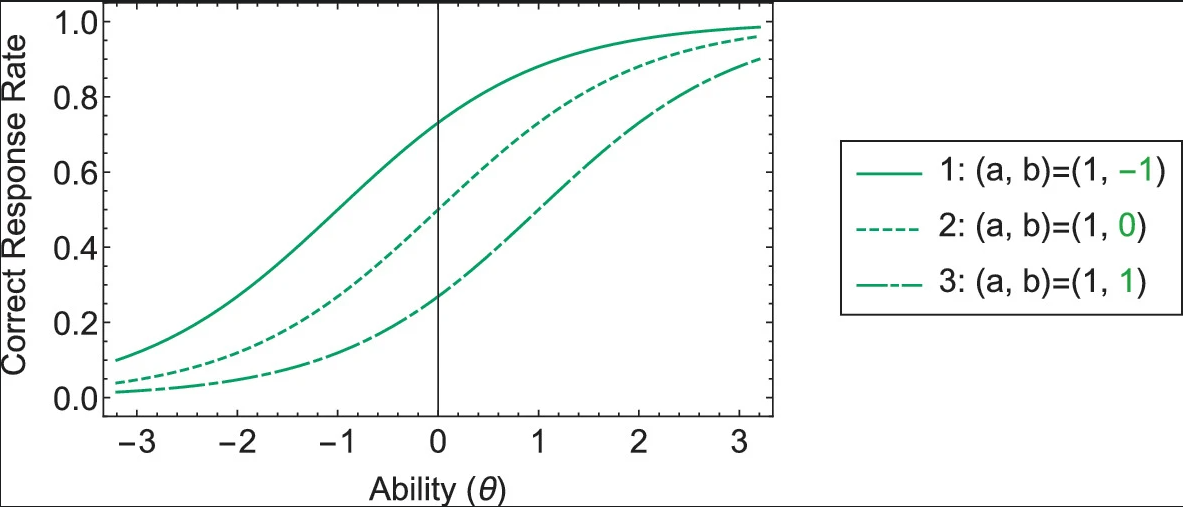
\includegraphics[scale=.5]{imagenes/IRTparambdifficulty.png}
	\caption{Probabilidad de responder correctamente para distintos valores del parámetro dificultad \textit{b}.}
	\label{ParamDifficulty}
\end{figure}


Es importante destacar que cada ítem discrimina mejor en torno a valores de $\theta$ que sean cercanos al parámetro de locación $b$. Además, un parámetro $a$ indica que el item es un mejor indicador para $\theta$, pero teniendo en consideración que este poder discriminativo funciona mejor cuando $\theta \approx b$. Por esta razón, cada pregunta por separado entrega información acerca del valor $\theta$ que se quiere obtener, de manera que las preguntas deben estar formuladas de tal manera que permitan distinguir distintos niveles del rasgo a evaluar \cite{TeoriaRespuestaAlItemPsicologia}.

Aplicando este modelo a una escala de Likert de formato ordinal, para cada pregunta se indican 4 parámetros b, para diferenciar entre los niveles 1) Muy en desacuerdo; 2) En desacuerdo; 3) Ni en desacuerdo ni de acuerdo; 4) De acuerdo y 5) Muy de acuerdo \cite{TeoriaRespuestaAlItemPsicologia, meegaplusQualityEvaluationPage}. De esta manera, a medida que $\theta$, la calidad de juego es mejor según \cite{meegaplusQualityEvaluationPage}, las respuestas más tenderán a ser del formato Muy de acuerdo, a excepción de algunas preguntas que no se incluyen en la valoración. El script de R utilizado para el cálculo de $\theta$ se encuentra disponible en \cite{meegaplusQualityEvaluationPage}.

Las fórmulas empleadas, demostraciones relacionadas con IRT o mostrar cómo afectan los distintos parámetros al resultado final está fuera del alcance de este estudio, principalmente porque los paquetes de R se encargan de realizar este trabajo. Para entender mejor cómo funciona este modelo por debajo, puede consultarse \cite{IRTShojima2022, CalderonStatisticalIRT}.

\subsection{Motores de videojuegos: Godot}

Existen diversos motores de videojuegos, como Unreal Engine \cite{UE}, Unity \cite{Unity} y Godot \cite{Godot}. Este último resalta por ser completamente gratuito, de código abierto y poseer una comunidad activa en el desarrollo del motor \cite{GodotGithubRepository}. Los motores de videojuegos ofrecen una ventaja significativa al proporcionar un entorno integrado que abarca diversas funcionalidades para diferentes profesionales. Por ejemplo, facilitan la integración de animaciones, efectos visuales, y trabajo con sonido. Además, incluyen bibliotecas incorporadas comúnmente utilizadas en videojuegos, como colisiones, texturizado, o composición de elementos, permitiendo la unificación de la representación visual, auditiva y programática de un personaje. Los motores de videojuegos también posibilitan la exportación de la aplicación a diversas plataformas sin necesidad de modificar el código \cite{GodotExport}.

Godot emplea principalmente dos lenguajes de programación: GDScript, similar a Python, y C\#. Ambos fueron utilizados en este trabajo. GDScript permite prototipar rápidamente debido a su simplicidad y estrecha integración con el motor. Por otro lado, C\# es más rápido, pero algunas características del motor no están completamente integradas en la versión utilizada durante este trabajo, que es la 3.5.2 \cite{GodotCSharpGDDifferences}.
